\documentclass{beamer}
\usetheme{Warsaw}  %% Themenwahl

\usepackage[utf8]{inputenc}
\usepackage[ngerman]{babel}
\usepackage{ngerman}
 
\title{Komponenten von SHA256}
\author{Lars Schmertmann}
\date{\today}
 
\begin{document}
\maketitle
\frame{\tableofcontents[currentsection]}
 
\section{Komponenten}
\subsection{Padding}
  \begin{frame}
    \frametitle{Padding}
    Allgemeines Padding:\\
    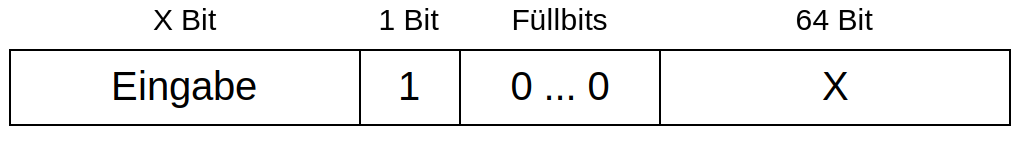
\includegraphics[width=300pt]{padding.pdf}\\
    \pause~\\
    Test:\\
    \includegraphics[width=300pt]{padding-allgemein.pdf}
  \end{frame}
\subsection{Funktionen}
  \begin{frame}
    \frametitle{Funktionen}
    \begin{itemize}
      \setlength{\itemsep}{20pt}
      \item Expansion
        \begin{itemize}
          \setlength{\itemsep}{10pt}
          \item $ SSIG0(x) = ROTR^{7}(x)~XOR~ROTR^{18}(x)~XOR~SHR^{3}(x) $
          \item $ SSIG1(x) = ROTR^{17}(x)~XOR~ROTR^{19}(x)~XOR~SHR^{10}(x) $
        \end{itemize}
      \item Computation
        \begin{itemize}
          \setlength{\itemsep}{10pt}
          \item $ CH( x, y, z) = (x~AND~y)~XOR~( (NOT~x)~AND~z) $
          \item $ MAJ( x, y, z) = (x~AND~y)~XOR~(x~AND~z)~XOR~(y~AND~z) $
          \item $ BSIG0(x) = ROTR^{2}(x)~XOR~ROTR^{13}(x)~XOR~ROTR^{22}(x) $
          \item $ BSIG1(x) = ROTR^{6}(x)~XOR~ROTR^{11}(x)~XOR~ROTR^{25}(x) $
        \end{itemize}
    \end{itemize}
  \end{frame}
\subsection{Expansion}
  \begin{frame} %%Eine Folie
    \frametitle{Expansion} %%Folientitel
    \begin{Definition} %%Definition
      Eine Definition
    \end{Definition}
  \end{frame}
\subsection{Computation}
  \begin{frame} %%Eine Folie
    \frametitle{Computation} %%Folientitel
    \begin{Definition} %%Definition
      Eine Definition
    \end{Definition}
  \end{frame}

\section{Bitcoin}
\subsection{Aufgabe}
\end{document}